% Tento soubor nahraďte vlastním souborem s přílohami (nadpisy níže jsou pouze pro příklad)
% This file should be replaced with your file with an appendices (headings below are examples only)

% Umístění obsahu paměťového média do příloh je vhodné konzultovat s vedoucím
% Placing of table of contents of the memory media here should be consulted with a supervisor
\chapter{Obsah přiložené SD karty}
\label{Att:Card}

Přiložená karta obsahuje:
\begin{itemize}
	\item \texttt{xpolas34-ECS.pdf} -- Text písemné zprávy.
	\item \texttt{xpolas34-ECS-tisk.pdf} -- Verze tohoto textu určená k tisku.
	\item \texttt{popis.txt} -- Popis obsahu karty a jak jej použít.
	\item \texttt{src\_text/}:
	\begin{itemize}
		\item Zdrojové texty této technické zprávy.
		\item \texttt{Poster/} -- Zdrojové texty plakátu.
	\end{itemize}
	\item \texttt{src/}:
	\begin{itemize}
		\item Zdrojové texty v programovacím jazyce \emph{C++}.
		\item \texttt{app/} -- Ukázková aplikace vytvořená pomocí entitního systému.
		\item \texttt{doc/}:
		\begin{itemize}
			\item \texttt{DoxyfileEntropy} -- Generátor dokumentace \emph{Doxygen}.
			\item \texttt{graph/} -- Skripty pro tvorbu grafů.
		\end{itemize}
		\item \texttt{Entropy/} -- Výsledek práce, knihovna \textbf{Entropy}.
		\item \texttt{include/} a \texttt{src/} -- Zdrojové kódy pomocných knihoven.
		\item \texttt{tests/} -- Zdrojové kódy testů a porovnání.
	\end{itemize}
	\item \texttt{exec/}
	\begin{itemize}
		\item Přeložené testovací aplikace, spustitelné na serveru \emph{Merlin}:
		\begin{itemize}
			\item \texttt{Comparison*} -- Porovnání entitních systémů
			\item \texttt{Test*} -- Testování knihovny \textbf{Entropy}.
			\item \texttt{gameTest} -- Implementace jednoduché aplikace.
			\item \texttt{res/} -- Zdroje pro spustitelný soubor \texttt{gameTest}.
		\end{itemize}
	\end{itemize}
	\item \texttt{archive/} -- Obsahuje záložní archivy s obsahem této karty.
	\item \texttt{*/external/} -- Všechny adresáře se jménem \texttt{external} obsahují externí knihovny, které nebyly vyvinuty autorem této práce.
\end{itemize}

\chapter{Manuál}
Tento manuál obsahuje informace o použití obsahu přiložené paměťové karty. Obsah této karty lze vidět v příloze \ref{Att:Card}.

\section*{Překlad}
Předem přeložené spustitelné soubory lze nalézt v adresáři \texttt{exec}. Jejich testování bylo provedeno na školním severu \emph{Merlin}.

Překlad pro jiné platformy lze provést následující sekvencí příkazů. Nástroje potřebné pro provedení překladu jsou:
\begin{itemize}
	\item Překladač jazyka \emph{C++}, který podporuje standard \emph{C++14}.
	\item CMake alespoň verze 3.1, pro překlad všech porovnávacích aplikací. Na serveru \emph{Merlin} byl použit \emph{cmake37}.
\end{itemize}
\noindent Výchozí adresář obsahuje kopii souborů z kořenového adresáře SD karty:
\begin{lstlisting}[basicstyle=\ttfamily]
  cd src && mkdir build && cd build
  cmake ../ -DCMAKE_BUILD_TYPE=Release
  # Nebo pro OS Windows.
  cmake ../ -DCMAKE_BUILD_TYPE=Release \
    -G "Visual Studio 15 2017 Win64"
  cmake --build . --config Release
\end{lstlisting}

Výsledkem překladu jsou spustitelné soubory a adresář \emph{res}, který obsahuje soubory nutné pro běh aplikace \texttt{gameTest}. Bližší informace k použití knihovny \textbf{Entropy} lze najít v~souborech \texttt{README.md} a \texttt{README\_CS.md} v adresáři \texttt{src/}.

\section*{Spustitelné soubory}

Mezi spustitelné soubory patří:
\begin{itemize}
	\item \texttt{gameTest} -- Jednoduchá grafická aplikace, která ukazuje využití \emph{entitního systému}. Vyžaduje přítomnost adresáře \texttt{res/}, který obsahuje soubory použité při běhu. Stiskem klávesy \emph{c} lze zapnout ovládání kamery.
	\item \texttt{Comparison*} -- Porovnání různých \emph{ECS} knihoven. Výstupem každého souboru je tabulka dat, kterou lze použít při tvorbě grafů. Testované scénáře lze specifikovat pomocí spuštění jednotlivých aplikací s parametry:
	\begin{itemize}
		\item \texttt{0 START DELTA MAX} -- Testování tvorby \emph{entit}.
		\item \texttt{1 ENTS REPEATS START DELTA MAX} -- Testování při daném procentu využití \emph{entit}.
		\item \texttt{2 ENTS REPEATS START DELTA MAX} -- Testování při daném procentu změn \emph{entit}.
		\item \texttt{3 ENTS REPEATS START DELTA MAX} -- Testování paralelního vykonávání. V tomto případě je použita paralelizace rozdělením \emph{entit}.
		\item \texttt{4 ENTS REPEATS START DELTA MAX} -- Testování paralelního vykonávání. V tomto případě je použita paralelizace použitím \emph{množin změn}.
		\item \texttt{5 START DELTA MAX REPEATS READ\_OPS TYPE RAND} -- Porovnání různých \emph{nosičů komponent} a velikostí daných \emph{komponent}. Typ je složen z typu \emph{nosiče} (\emph{m}, \emph{ml} a \emph{l}) a typu \emph{komponenty} (\emph{s}, \emph{m} a \emph{l}).
		\item \texttt{6 ENTS REPEATS THREADS START DELTA MAX} -- Porovnání paralelizace pro případ jednoduchého \emph{systému} s daným procentem využitých \emph{entit}.
		\item \texttt{7 ENTS REPEATS THREADS START DELTA MAX} -- Porovnání paralelizace pro případ jednoduchého \emph{systému} s daným procentem změněných \emph{entit}.
	\end{itemize}
	\item \texttt{Test*} -- Testování částí knihovny \textbf{Entropy}. Výstupem je seznam testovaných scénářů, případně informace o tom, které nebyly splněny. Pokud všechny testy v daném soubory byly splněny, program vrací hodnotu 0. Jednotlivé soubory mají následující funkce: 
	\begin{itemize}
		\item \texttt{TestEntropy} -- Základní testy jednotlivých částí \emph{entitního systému}.
		\item \texttt{TestEntropyMisc} -- Testování obecných datových struktur.
		\item \texttt{TestEntropyParallel} -- Testování vícevláknového použití \emph{entitního systému}.
		\item \texttt{TestEntropyPerformance} -- Výkonnostní testy.
		\item \texttt{TestEntropySandbox} -- Testování vlastností výsledného \emph{entitního systému}.
	\end{itemize}
\end{itemize}

\section*{Generování grafů}
Pro generování grafů je nutné, aby spustitelné soubory \texttt{Comparison*} byly obsaženy v adresáři \emph{src/build/}. Dále je nutné, aby systém obsahoval nástroj \texttt{R}, spustitelný voláním \texttt{Rscript}. Pro správnou funkci skriptu jsou nutná \emph{root} práva, pro spuštění testovaných aplikaci s vyšší prioritou. Generaci grafů lze spustit následovně:
\begin{lstlisting}[basicstyle=\ttfamily]
  cd src/doc/graph
  ./makeGraphs.sh
\end{lstlisting}

\chapter{Plakát}
\begin{center}
	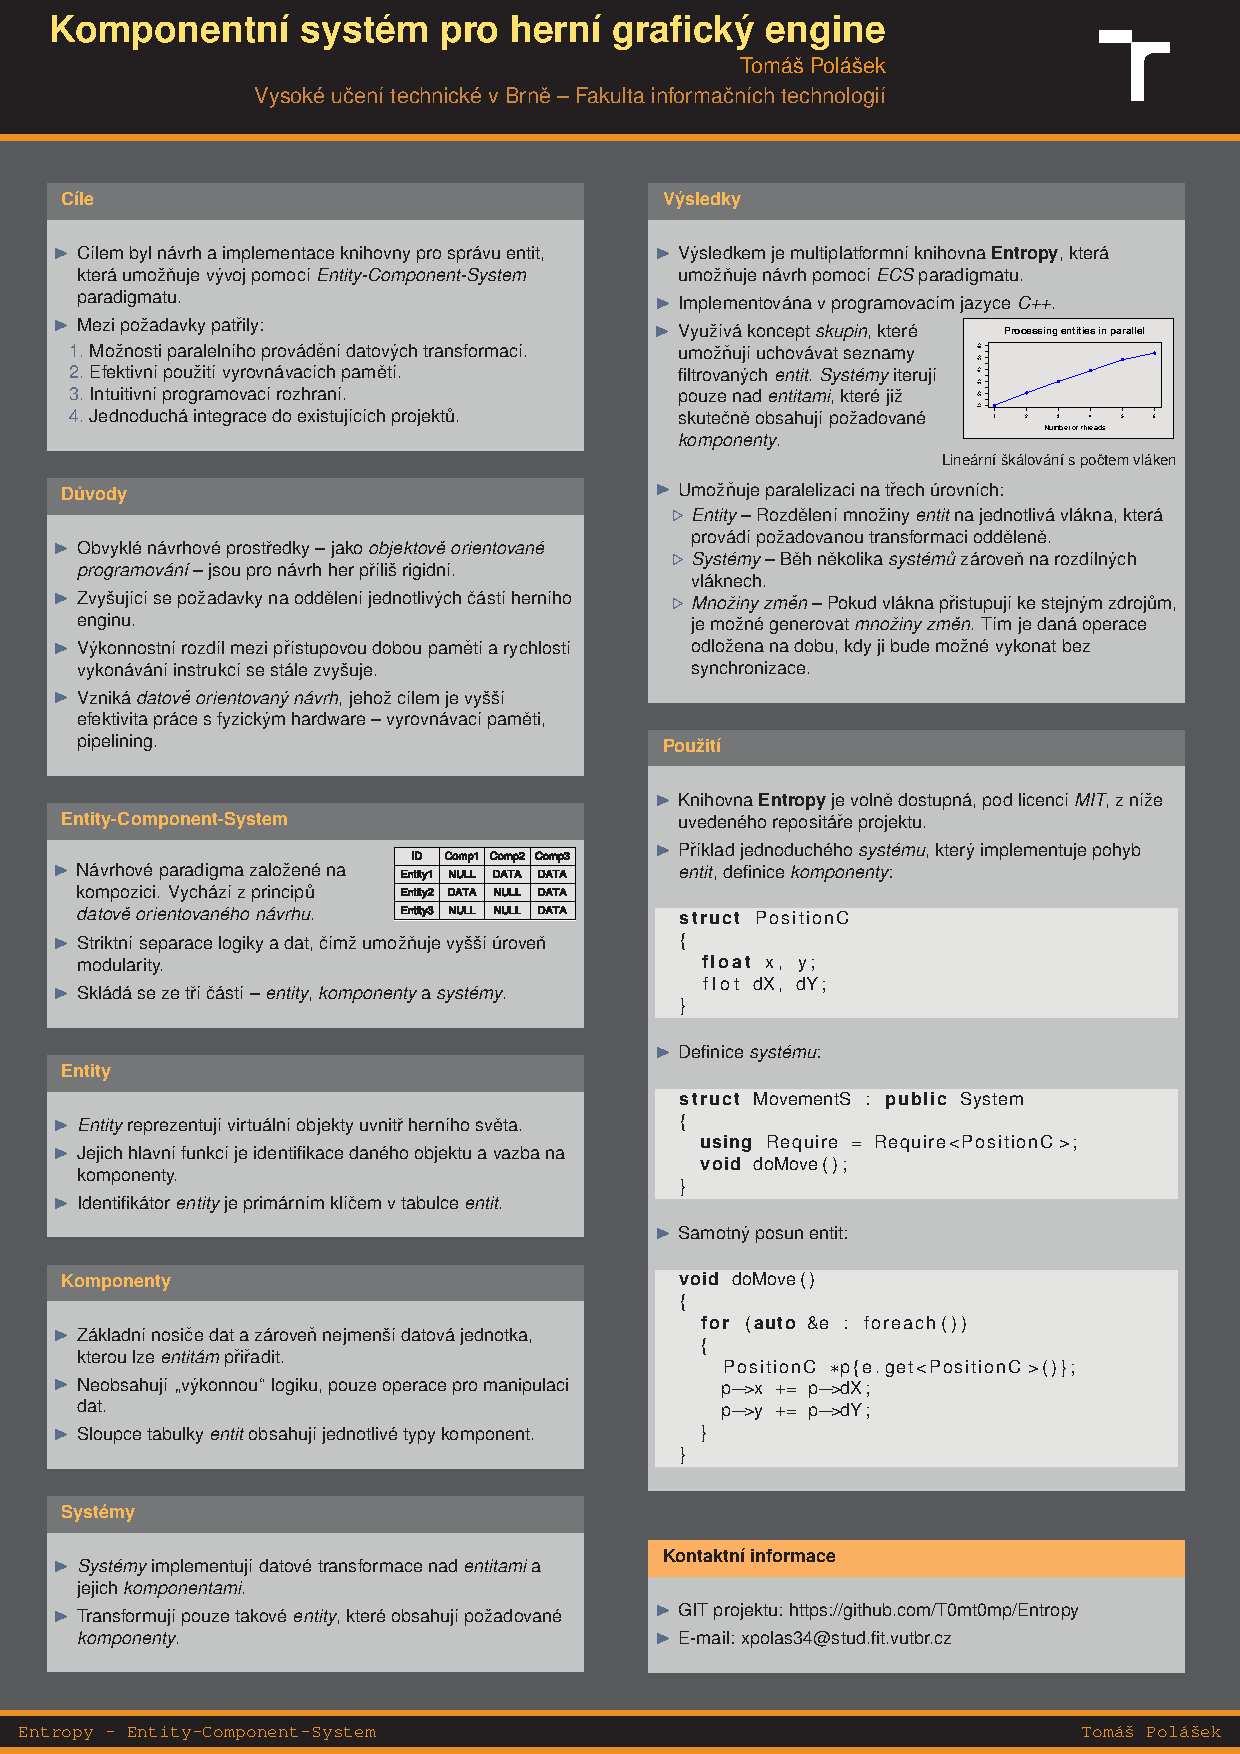
\includegraphics[scale=0.5]{poster.pdf}
\end{center}

\chapter{Použití knihovny}

\section*{Co je Entropy}

\textbf{Entropy} je knihovna napsaná v programovacím jazyce \emph{C++}, která umožňuje návrh aplikací za použití \emph{Entity-Component-System} paradigmatu. Knihovna je volně k dispozici, pod \emph{MIT} licencí, v repositáři \href{https://github.com/T0mt0mp/Entropy}{GIT}. 

\section*{Použití knihovny}

\subsection*{Požadavky}

Pro správnou funkci vyžaduje knihovna následující nástroje: 
\begin{itemize}
	\item Překladač jazyka \emph{C++}, který podporuje standard jazyka \emph{C++14} -- mezi testované překladače patří GCC 6.3.1, Clang 3.9.1 a MSVC 19.10
	\item (volitelné) CMake -- alespoň verze 2.8 (3.1 pro překlad porovnání, kvůli knihovně EntityX)
\end{itemize}

\subsection*{Stažení}

Nejjednodušším způsobem, jak získat knihovnu \textbf{Entropy}, je klonováním jejího repositáře:

\begin{lstlisting}[basicstyle=\ttfamily]
  mkdir Entropy
  git clone https://github.com/T0mt0mp/Entropy Entropy
  cd Entropy
  git submodule update --init --recursive
\end{lstlisting}

\subsection*{Překlad testů}

Součástí knihovny \textbf{Entropy} jsou testy, které lze přeložit pomocí systému \emph{CMake}. 

\begin{lstlisting}[basicstyle=\ttfamily]
  mkdir build && cd build
  cmake ../ -DCMAKE_BUILD_TYPE=Release
\end{lstlisting}
nebo pro operační systém Windows:
\begin{lstlisting}[basicstyle=\ttfamily]
  cmake ../ -DCMAKE_BUILD_TYPE=Release \
    -G "Visual Studio 15 2017 Win64"
\end{lstlisting}
\pagebreak
potom lze pro překlad použít:
\begin{lstlisting}[basicstyle=\ttfamily]
  cmake --build . --config Release
\end{lstlisting}

\noindent Výsledkem jsou spustitelné soubory v adresáři \texttt{build}, nebo \texttt{Release}:
\begin{itemize}
	\item \texttt{Comparison*} -- Porovnání různých volně dostupných knihoven.
	\item \texttt{Test*} -- Testy knihovny \textbf{Entropy}.
	\item \texttt{gameTest} -- Testovací implementaci hry za použití knihovny \textbf{Entropy}.
\end{itemize}

\subsection*{Instalace}

Po stažení knihovny ji lze nainstalovat do adresáře \texttt{/usr/local/include} následující sekvencí příkazů: 

%\begin{lstlisting}[language=C++]
\begin{lstlisting}[basicstyle=\ttfamily]
  mkdir build && cd build
  cmake ../Entropy/ && make install
\end{lstlisting}

\noindent Alternativně je možné manuálně nakopírovat obsah adresáře \texttt{Entropy/include/} (obsahuje složku \texttt{Entropy}) do systémového \texttt{include}, nebo jiného adresáře, kde ji překladač najde.

\subsection*{Základy}

Před jejím použitím je nutno knihovnu přidat do zdrojového kódu, pomocí direktivy \texttt{include}:

\begin{lstlisting}[backgroundcolor = \color{lightgray}, language = C++, xleftmargin = 2cm, framexleftmargin = 1em, tabsize=4]
#include <Entropy/Entropy.h>
\end{lstlisting}

\subsubsection*{Universe}

Středem knihovny \textbf{Entropy} je třída \textbf{Universe}, která umožňuje komunikaci s entitním systémem. Z této třídy je třeba nejdříve podědit což umožňuje existenci několika oddělených světů:

\begin{lstlisting}[backgroundcolor = \color{lightgray}, language = C++, xleftmargin = 2cm, framexleftmargin = 1em, tabsize=4]
class MyUniverse : public ent::Universe<MyUniverse>
{ };
\end{lstlisting}

\noindent Potom již lze vytvořit instance daného vesmíru:

\begin{lstlisting}[backgroundcolor = \color{lightgray}, language = C++, xleftmargin = 2cm, framexleftmargin = 1em, tabsize=4]
MyUniverse u;
\end{lstlisting}

\subsubsection*{Entity}

\emph{Entity} jsou v knihovně \textbf{Entropy} jednoduché číselné identifikátory, kterým je možné přiřadit 0-1 \emph{komponent}. \emph{Entity} se mohou nacházet ve dvou stavech -- aktivní a neaktivní. Tvorba nových entit je možná skrz třídu \textbf{Universe}:

\begin{lstlisting}[backgroundcolor = \color{lightgray}, language = C++, xleftmargin = 2cm, framexleftmargin = 1em, tabsize=4]
using Entity = MyUniverse::EntityT;
Entity e = u.createEntity();
\end{lstlisting}

\noindent \emph{Entity} je dále možné zničit, použitím metody \texttt{destroy}:
\begin{lstlisting}[backgroundcolor = \color{lightgray}, language = C++, xleftmargin = 2cm, framexleftmargin = 1em, tabsize=4]
e.destroy();
\end{lstlisting}

\noindent Informaci, zda je \emph{entita} platná lze získat metodou \texttt{valid}. \emph{Entity} se stává nevalidní ve chvíli, kdy je zničena.

\subsubsection*{Komponenty}

\emph{Komponenty} jsou základními nosiči dat v \emph{ECS}. Nové typy \emph{komponent} lze definovat následovně:

\begin{lstlisting}[backgroundcolor = \color{lightgray}, language = C++, xleftmargin = 2cm, framexleftmargin = 1em, tabsize=4]
struct PositionC
{
	float x, y;
};
\end{lstlisting}

\noindent Aby třída, nebo struktura, mohla být považována za \emph{komponentu}, musí splňovat následující požadavky. Musí obsahovat výchozí konstruktor -- konstruktor bez parametrů. Kromě toho může obsahovat neomezený počet dalších konstruktorů, kterým lze předávat parametry při přidání \emph{komponenty}. 

Každý typ \emph{komponent} v knihovně \textbf{Entropy} má vlastní tzv. \emph{nosič komponent}. Nové typy \emph{nosičů} lze definovat skrz dědění třídy \textbf{BaseComponentHolder} a implementaci všech virtuálních metod. Knihovna \textbf{Entropy} obsahuje tři typy předdefinovaných nosičů:

\begin{itemize}
	\item \textbf{ComponentHolder} -- Výchozí nosič pro komponenty, které nemají specifikovaný jiný. Používá \texttt{std::map}. Tento nosič je výhodný v případech, kdy nejsou entity, které obsahují daný typ komponenty nijak seřazené.
	\item \textbf{ComponentHolderMapList} -- Používá \texttt{std::map}, který mapuje entity do souvislého pole komponent.
	\item \textbf{ComponentHolderList} -- Používá pole, do kterého jsou přímo namapovány identifikátory entit. Tento nosič je výhodný pro případy, kdy každá entita obsahuje daný typ komponent.
\end{itemize}

\noindent Specifikaci nosiče komponent lze provést následujícím způsobem:

\begin{lstlisting}[backgroundcolor = \color{lightgray}, language = C++, xleftmargin = 2cm, framexleftmargin = 1em, tabsize=4]
struct PositionC
{
	using HolderT = ent::ComponentHolderList<PositionC>;
	
	PositionC(float px, float py) :
		x{px}, y{py} { }
	PositionC() : 
		x{0.0f}, y{0.0f}
	float x, y;
};
\end{lstlisting}

Nad entitami lze provádět operace, které ovlivňují jaké komponenty daná entita obsahuje. Mezi tyto operace patří -- přidání (\texttt{add}), odebrání (\texttt{remove}), získání komponenty (\texttt{get}) a získání přítomnosti (\texttt{has}). Příklad použití těchto metod je následující:

\begin{lstlisting}[backgroundcolor = \color{lightgray}, language = C++, xleftmargin = 2cm, framexleftmargin = 1em, tabsize=4]
Entity e = u.createEntity();
e.add<PositionC>();
e.remove<PositionC>();
e.has<PositionC>();		// -> false
e.add<PositionC>(1.0f, 2.0f);
e.has<PositionC>();		// -> true
e.get<PositionC>->y;	// -> 2.0f
\end{lstlisting}

\subsubsection*{Systémy}

\emph{Systémy} umožňují iteraci nad entitami, tedy i nad komponentami, které vyhovují danému filtru. Jelikož komponenty neobsahují žádnou logiku, \emph{systémy} plní funkci tvorby akcí. Pokud bychom chtěli vytvořit systém, který bude iterovat nad entitami s komponenty typu \textbf{positionC} a \textbf{MovementC}, vypadala by jeho deklarace následovně:

\begin{lstlisting}[backgroundcolor = \color{lightgray}, language = C++, xleftmargin = 2cm, framexleftmargin = 1em, tabsize=4]
class MovementS : public MyUniverse::SystemT
{
	using Require = ent::Require<PositionC, MovementC>;
	using Reject = ent::Reject<>;
public:
	void doMove();
};
\end{lstlisting}

\noindent V tomto případě není \texttt{Reject} nutné, jelikož výchozí hodnota obou typů je prázdný typový seznam. Implementace samotné akce by mohla vypadat následovně:

\begin{lstlisting}[backgroundcolor = \color{lightgray}, language = C++, xleftmargin = 2cm, framexleftmargin = 1em, tabsize=4]
void MovementS::doMove()
{
	for (auto &e : foreach())
	{
		PositionC *p{e.get<PositionC>()};
		MovementC *m{e.get<MovementC}()};
		p->x += m->dX;
		p->y += m->dY;
	}
}
\end{lstlisting}

\noindent Děděná třída \emph{System}, obsahuje 3 metody -- \texttt{foreach}, \texttt{foreachAdded} a \texttt{foreachRemoved} -- díky kterým lze iterovat před entity vyhovující specifikovanému filtru. \emph{Systémy} lze přidat danému vesmíru voláním metody \texttt{addSystem<S>}.

\subsubsection*{Kontrolní tok}

Důležitou součástí knihovny \textbf{Entropy} je tok kontroly, který postupuje následujícím způsobem: 
\begin{enumerate}
	\item Vytvoření instance třídy \textbf{Universe}.
	\item Registrace komponent, metodou \texttt{registerComponent<C>}. Tento krok je možný pouze před inicializací!
	\item Inicializace vesmíru zavoláním metody \texttt{init} na dané instanci třídy \textbf{Universe}.
	\item Následně je již možná práce s entitním systémem -- přidávání \emph{systémů}, tvorba entit apod. \label{Enum:Work}
	\item Kdykoliv lze z předchozí fáze přejít do fáze \emph{obnovy}, kdy je obnovena konzistence celého entitního systému. Po dokončení se systém vrací do kroku \ref{Enum:Work}.
\end{enumerate}

\noindent Součástí \emph{obnovovací} fáze je také aktualizace seznamů, nad kterými \emph{systémy} iterují. 

%\chapter{Konfigurační soubor} % Configuration file

%\chapter{RelaxNG Schéma konfiguračního souboru} % Scheme of RelaxNG configuration file

%\chapter{Plakát} % poster
